\documentclass[12pt,a4paper]{article}
\usepackage[margin=0.75in]{geometry}
\usepackage{amsmath, amsfonts, amssymb,amsthm,epsfig,epstopdf,titling,url,array}
\usepackage{subfig}
\usepackage{graphicx}
\usepackage{hyperref}
\usepackage{amsbsy}
\usepackage{epsfig}
\usepackage{subfig}
\usepackage{bm}
\usepackage{xspace}
\usepackage{color}
\usepackage{colortbl}
\usepackage{subfloat}
\usepackage{lineno}
\usepackage{authblk}
\usepackage[section]{placeins}
\DeclareMathOperator{\Tr}{Tr}
% \renewcommand{\familydefault}{cmss}
\usepackage{setspace}


\setlength{\parindent}{0.5cm}
\setlength{\parskip}{6pt}

    \newcommand{\beginsupplement}{%
        \setcounter{table}{0}
        \renewcommand{\thetable}{\arabic{table}}%
        \setcounter{figure}{0}
        \renewcommand{\thefigure}{\arabic{figure}}%
        \setcounter{equation}{0}
        \renewcommand{\theequation}{\arabic{equation}}%
     }


\newcommand{\MH}[1]{{\color{red}#1}}
\newcommand{\cc}[1]{{\color{blue}#1}}
\newcommand{\js}[1]{{\color{green}#1}}
\newcommand{\comment}[1]{}

\begin{document}

\title{Measles Outbreaks in Canada: a short modelling study
}


\author[1]{Jennifer McNichol}
\author[1]{Javad Valizadeh}
\author[1]{Samara Chaudhury}
\author[1,*]{Caroline Colijn}

\affil[1]{Department of Mathematics, Simon Fraser University, Burnaby, BC, Canada, V5A 1S6}
\affil[*]{Corresponding author: ccolijn@sfu.ca}

\maketitle

\section{Introduction}

Measles is an infectious disease caused by the measles virus. It can cause serious complications, including ear infections and diarrhoea, but also pneumonia, encephalitis and in rarer cases, death. While measles can be serious in any age group, those under 5 years old, over 20, and those who are immune-compromised are most at risk. Measles is highly contagious, with a basic reproduction number of 12-18.
In this brief report we use a simple stochastic simulation model to explore how large measles outbreaks in Canada could be, based on past outbreak sizes in similar populations, parameters for the transmissibility of measles and the course of infection, and Canadian heterogenous vaccination rates.

\section{Methods}
Vaccination in Canada
Canada has high levels of measles vaccination overall, with Statistics Canada reporting 90\% or higher coverage of recommended measles vaccines in the 2017-2021 period (https://www150.statcan.gc.ca/t1/tbl1/en/tv.action?pid=1310087001). However, there is considerable variability between regions and communities, with some areas, schools or geographies vulnerable to measles outbreaks due to considerably lower vaccination rates. Table \ref{tab:vaxrequire} lists provincial and territorial data sources and whether vaccination is required or recommended for school-age children. We show some of these data in Figures 1 and 1.


% INSERT TABLE 1  from the google doc
\begin{table}[h!]
  \centering

  \caption[Vaccination requirements by province]{Vaccination requirements in schools in Canadian regions, with data and/or reports of vaccination rates}
  \label{tab:vaxrequire}
  \begin{tabular}{lp{3cm}p{10cm}}
	  \bf{Province} & \bf{Required to start school?} & \bf{Coverage rates \& provincial reports}                                                                                                                                                \\ \hline
NFLD     & Recommended               & A recent news interview states 95\% of the pop https://www.cbc.ca/player/play/2308385347572\#:$\sim$:text=The\%20key\%20to\%20protection\%20is,was\%20a\%20traveller\%20in\%202017. \\ \hline
PEI      & Recommended               & Rates prior to grade 1 entry for 2022-2023: https://www.princeedwardisland.ca/en/publication/childhood-immunization-rates-year-20222023-school-age                                  \\ \hline
NS       & Recommended               & Not found                                                                                                                                                                      \\ \hline
NB       & Required                  & NA                                                                                                                                                                                  \\ \hline
QC       & Recommended               & Data not found, but some news reports suggest some schools as low as 75\%                                                                                                                \\ \hline
ON       & Required                  & NA                                                                                                                                                                                  \\ \hline
MB       & Required                  & NA                                                                                                                                                                                  \\ \hline
SK       & Recommended               & https://www.saskatchewan.ca/residents/health/accessing-health-care-services/immunization-services/immunization-rates-in-saskatchewan                                                \\ \hline
AB       & Recommended               & http://www.ahw.gov.ab.ca/IHDA\_Retrieval/selectSubCategory.do                                                                                                                       \\ \hline
BC       & Recommended               & http://www.bccdc.ca/health-professionals/data-reports/immunizations                                                                                                                 \\ \hline
Yukon    & Recommended               & Not found                                                                                                                                                                           \\ \hline
Nunavut  & Recommended               & Not found                                                                                                                                                                           \\ \hline
NWT      & Recommended               & Not found
\end{tabular}
\end{table}

\begin{figure}[h]
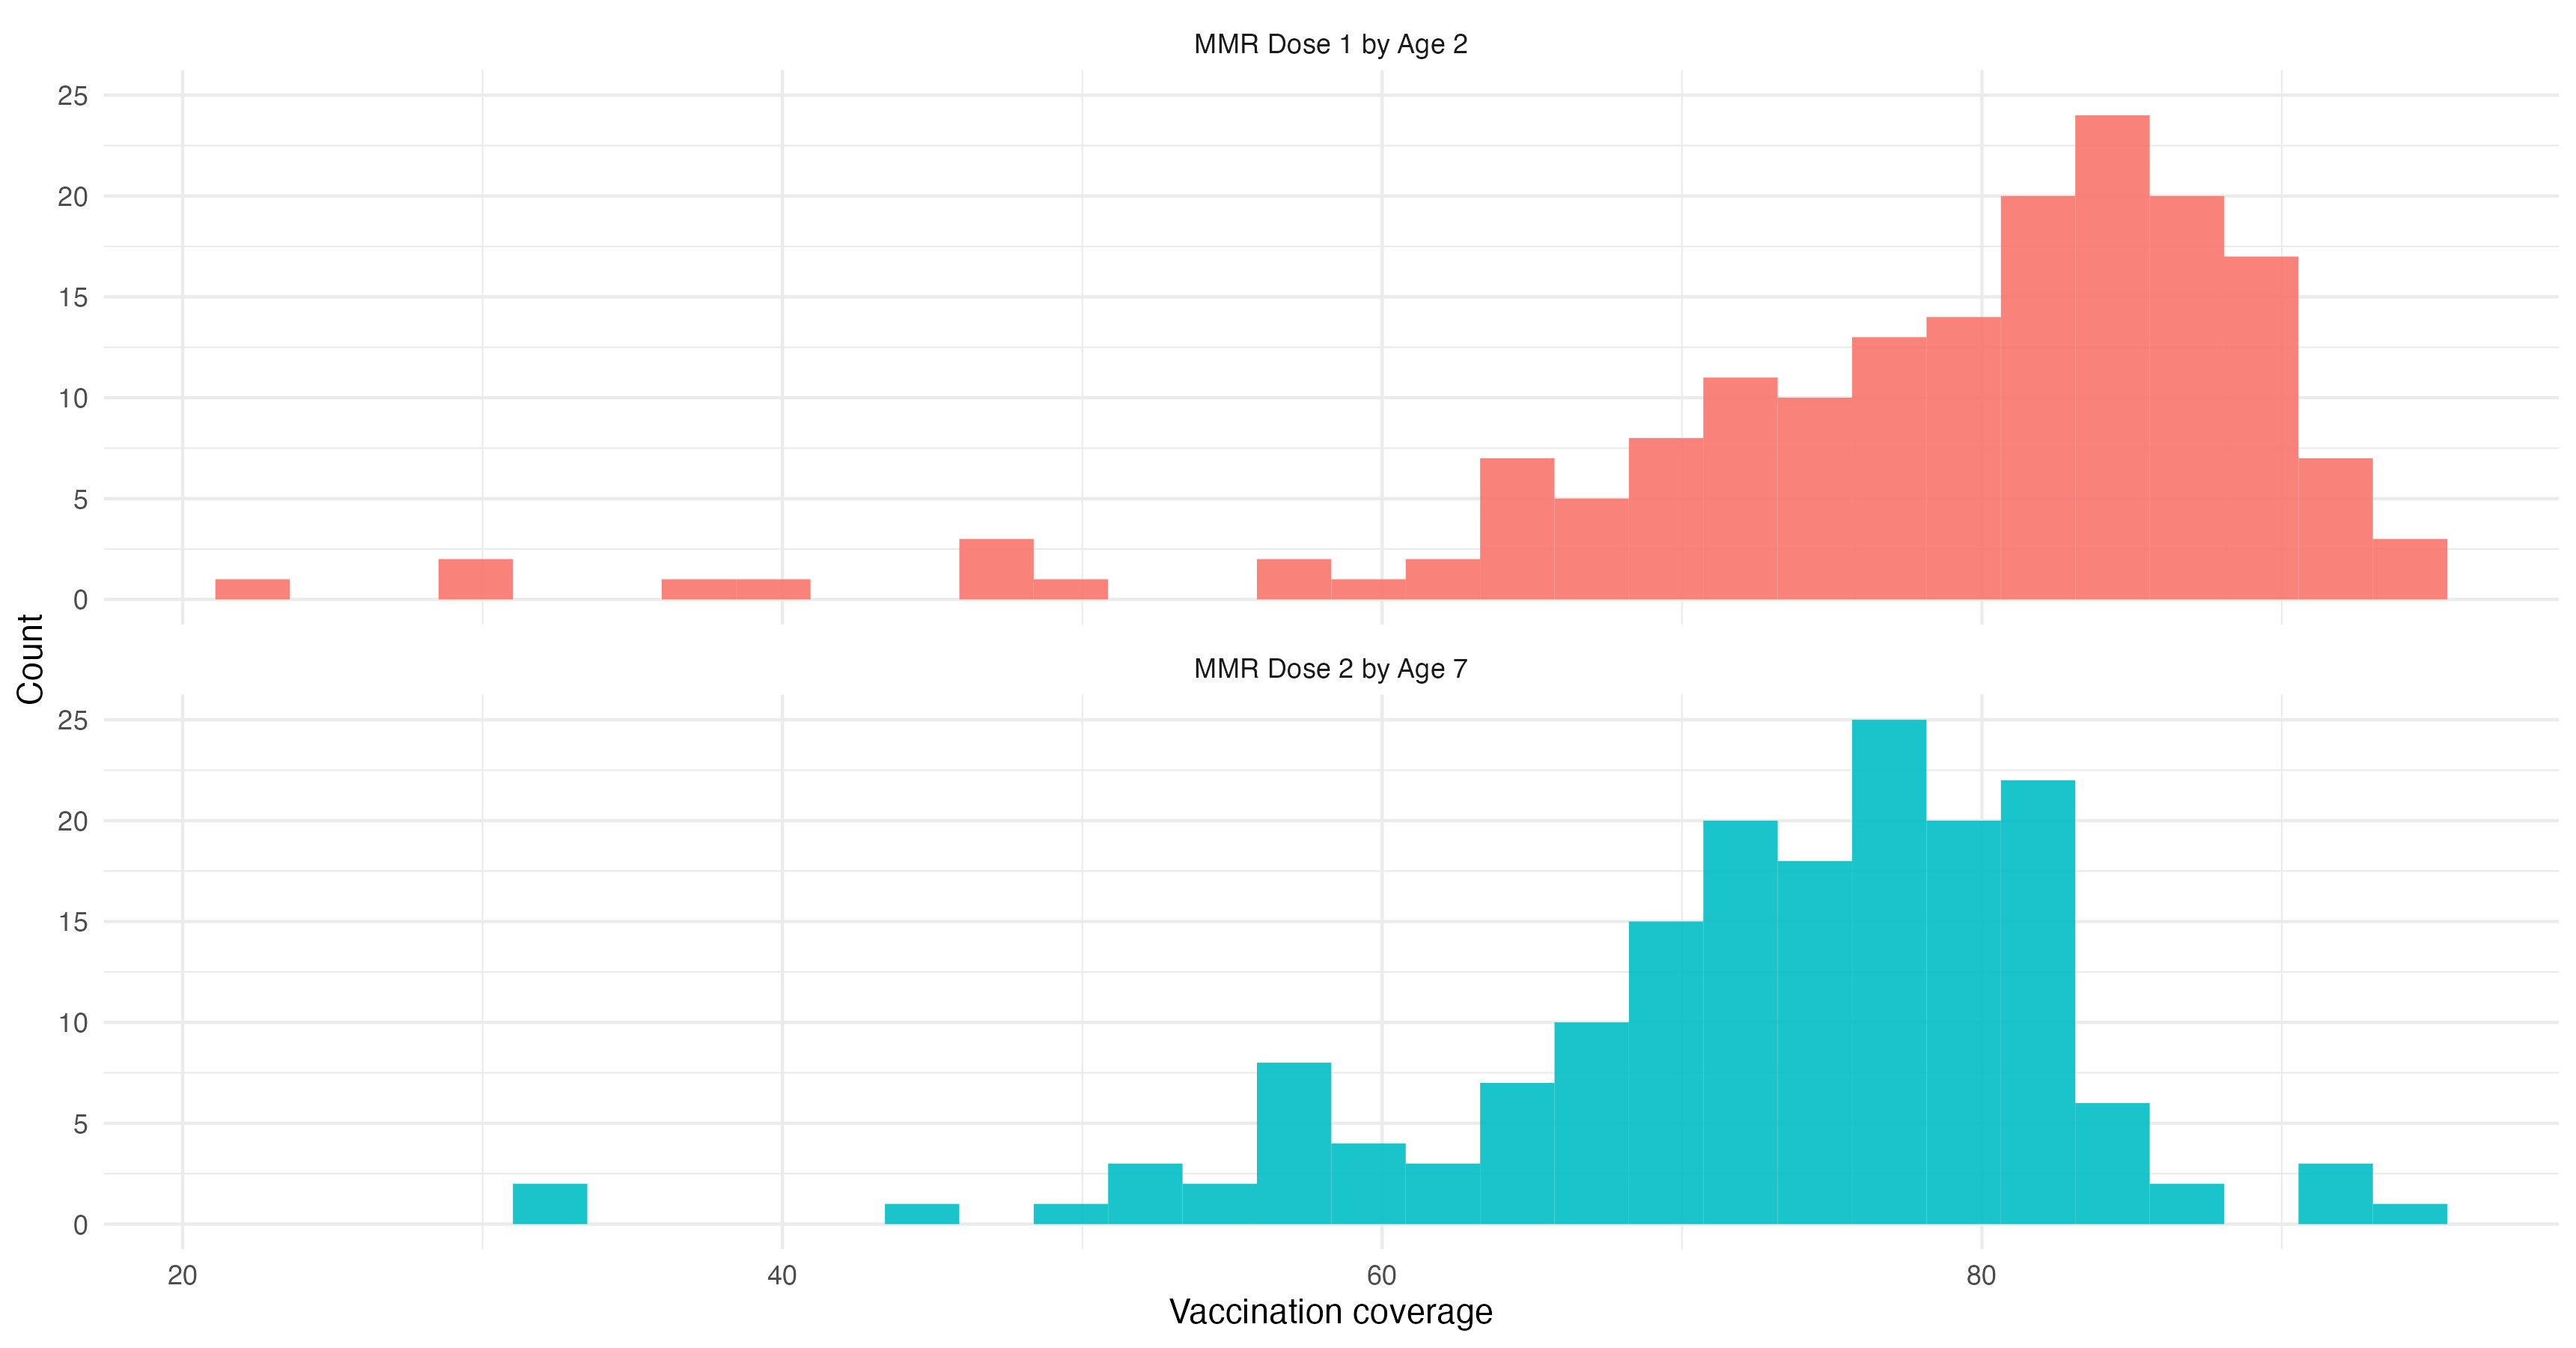
\includegraphics[width=\linewidth]{report-figs/f1.png}
\caption{AB coverage}
\label{fig:abcov}
\end{figure}

Similarly, British Columbia’s regional MMR coverage ranges from 77 to 89\% at age 2 and 75 to 92\% at age 7, as of 2020 (the most recent year for which data are available). (http://www.bccdc.ca/health-professionals/data-reports/immunizations). Saskatchewan reports very high vaccination levels for measles, with all jurisdictions over 85\% coverage and the majority over 90\% (Figure 2).

\begin{figure}[!h]
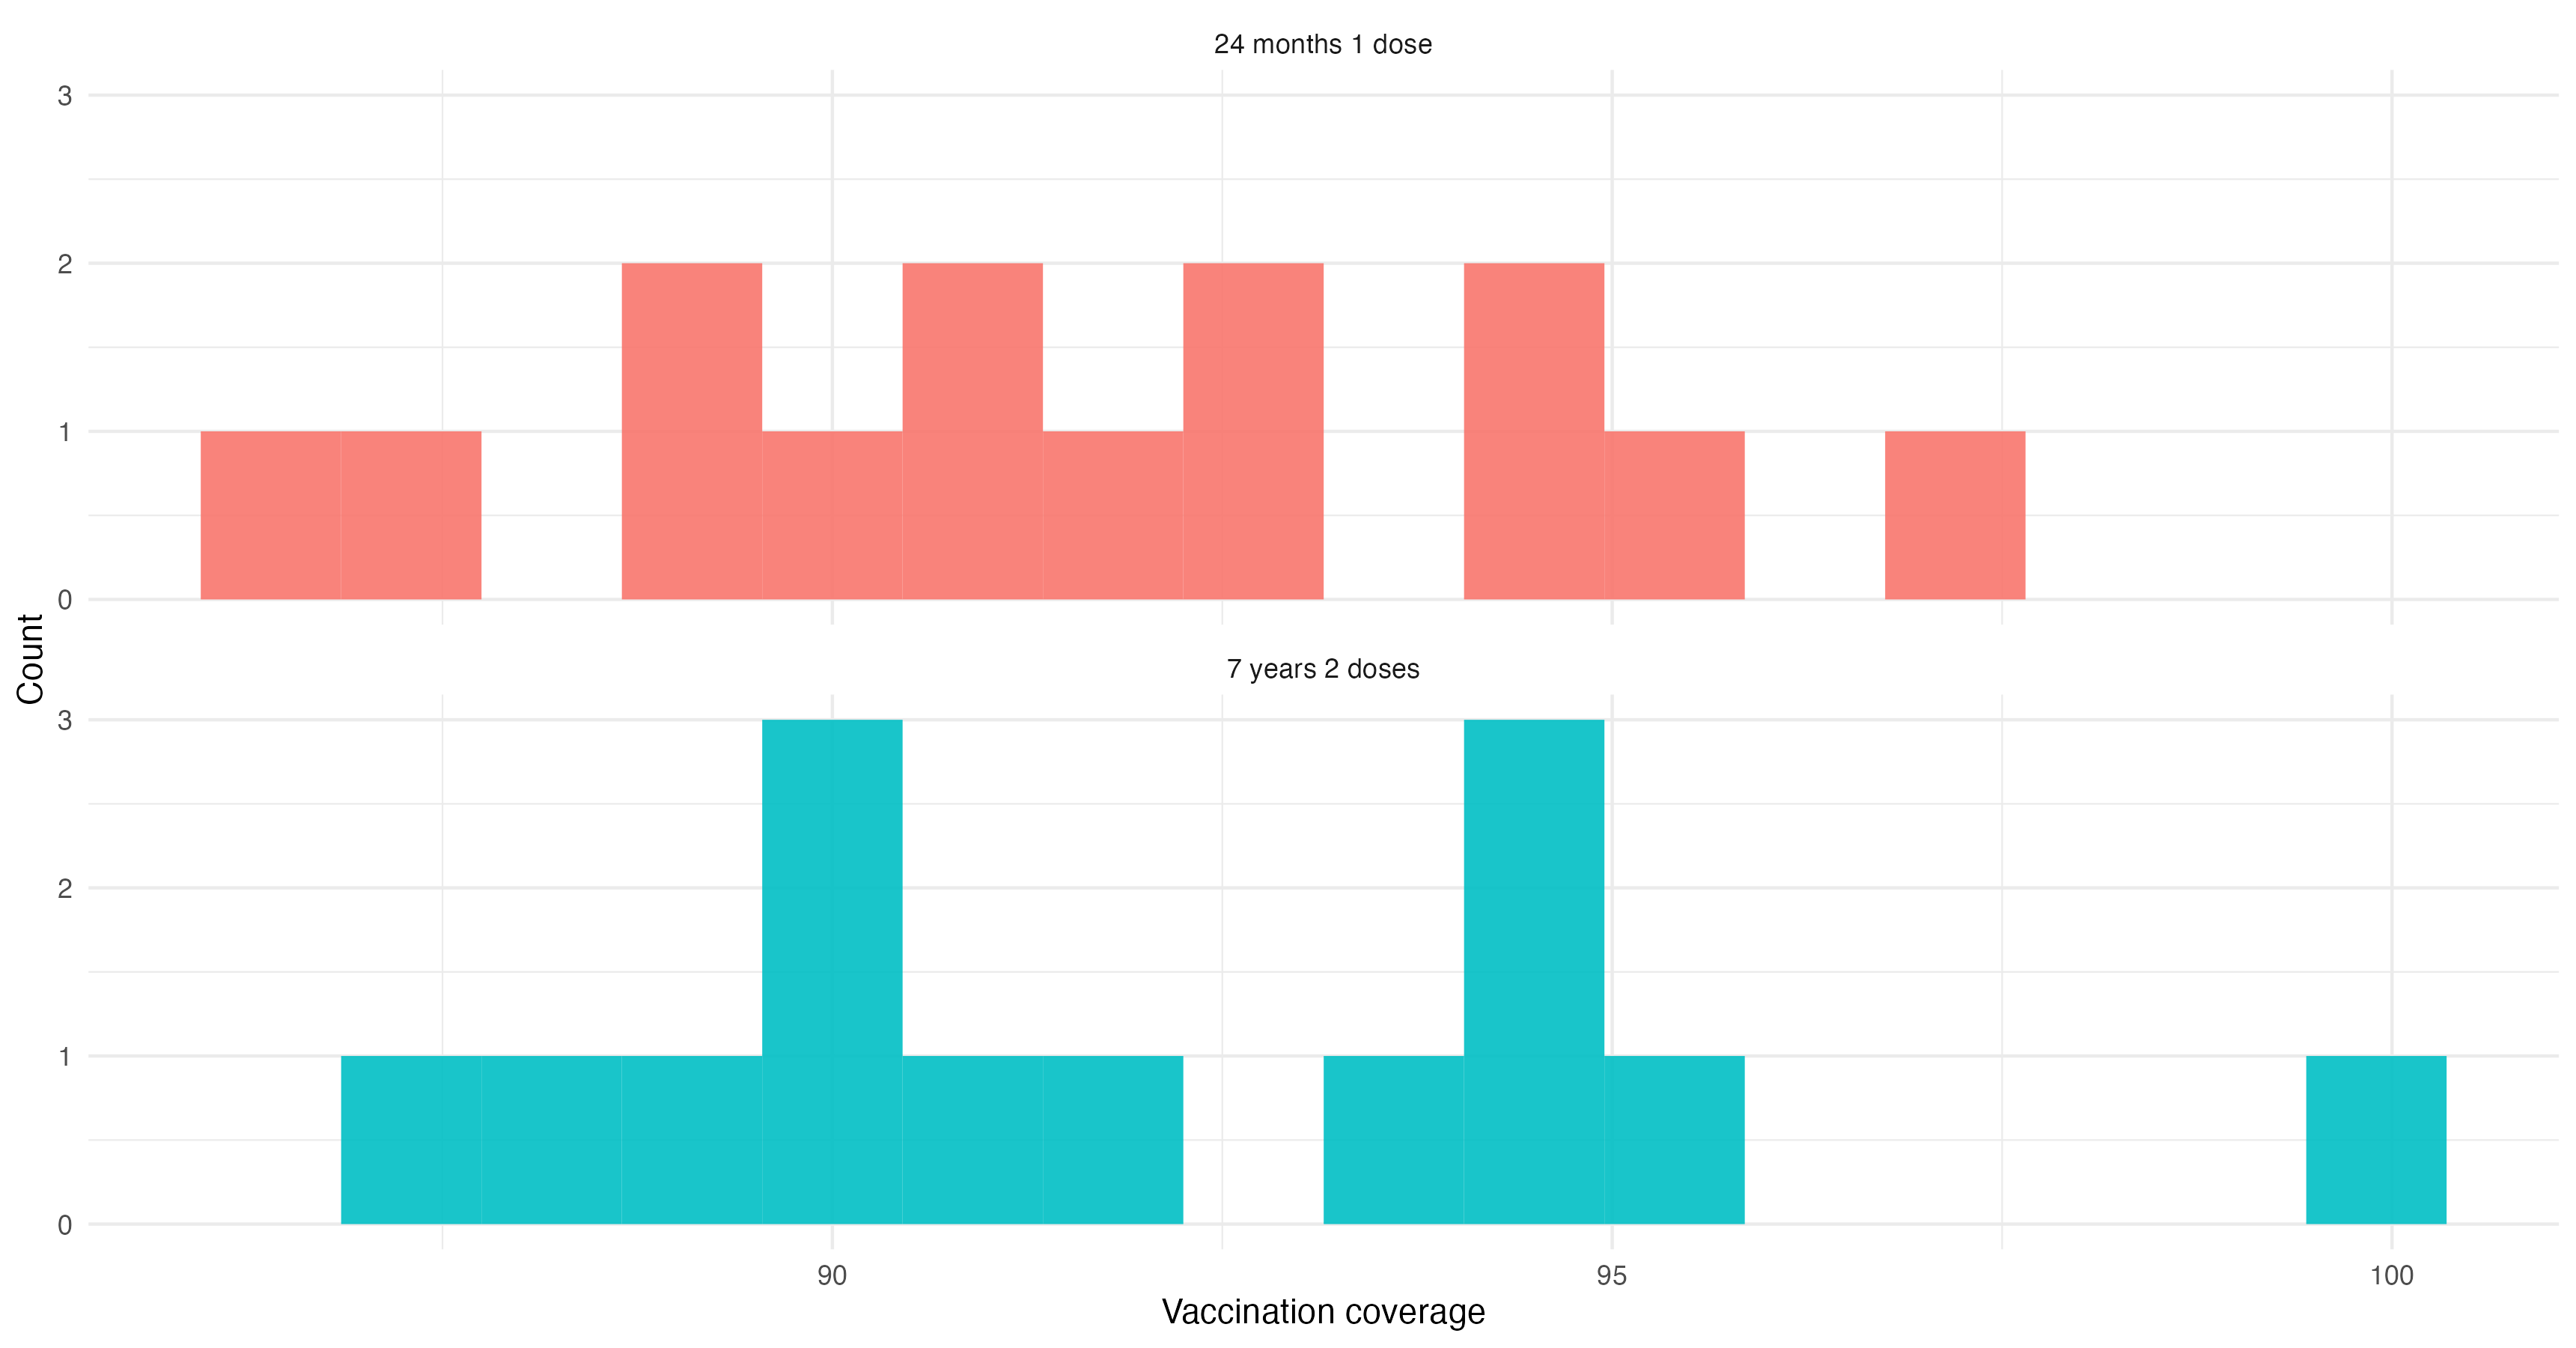
\includegraphics[width=\linewidth]{report-figs/f2.png}
\label{fig:skcov}
\caption{SK coverage}
\end{figure}

In some jurisdictions, school data are also available. For example, Figure 3 shows Vancouver School Board’s vaccination data, with occasional very low reported rates, and the majority of schools with at least 65\% coverage.

\begin{figure}[h!]
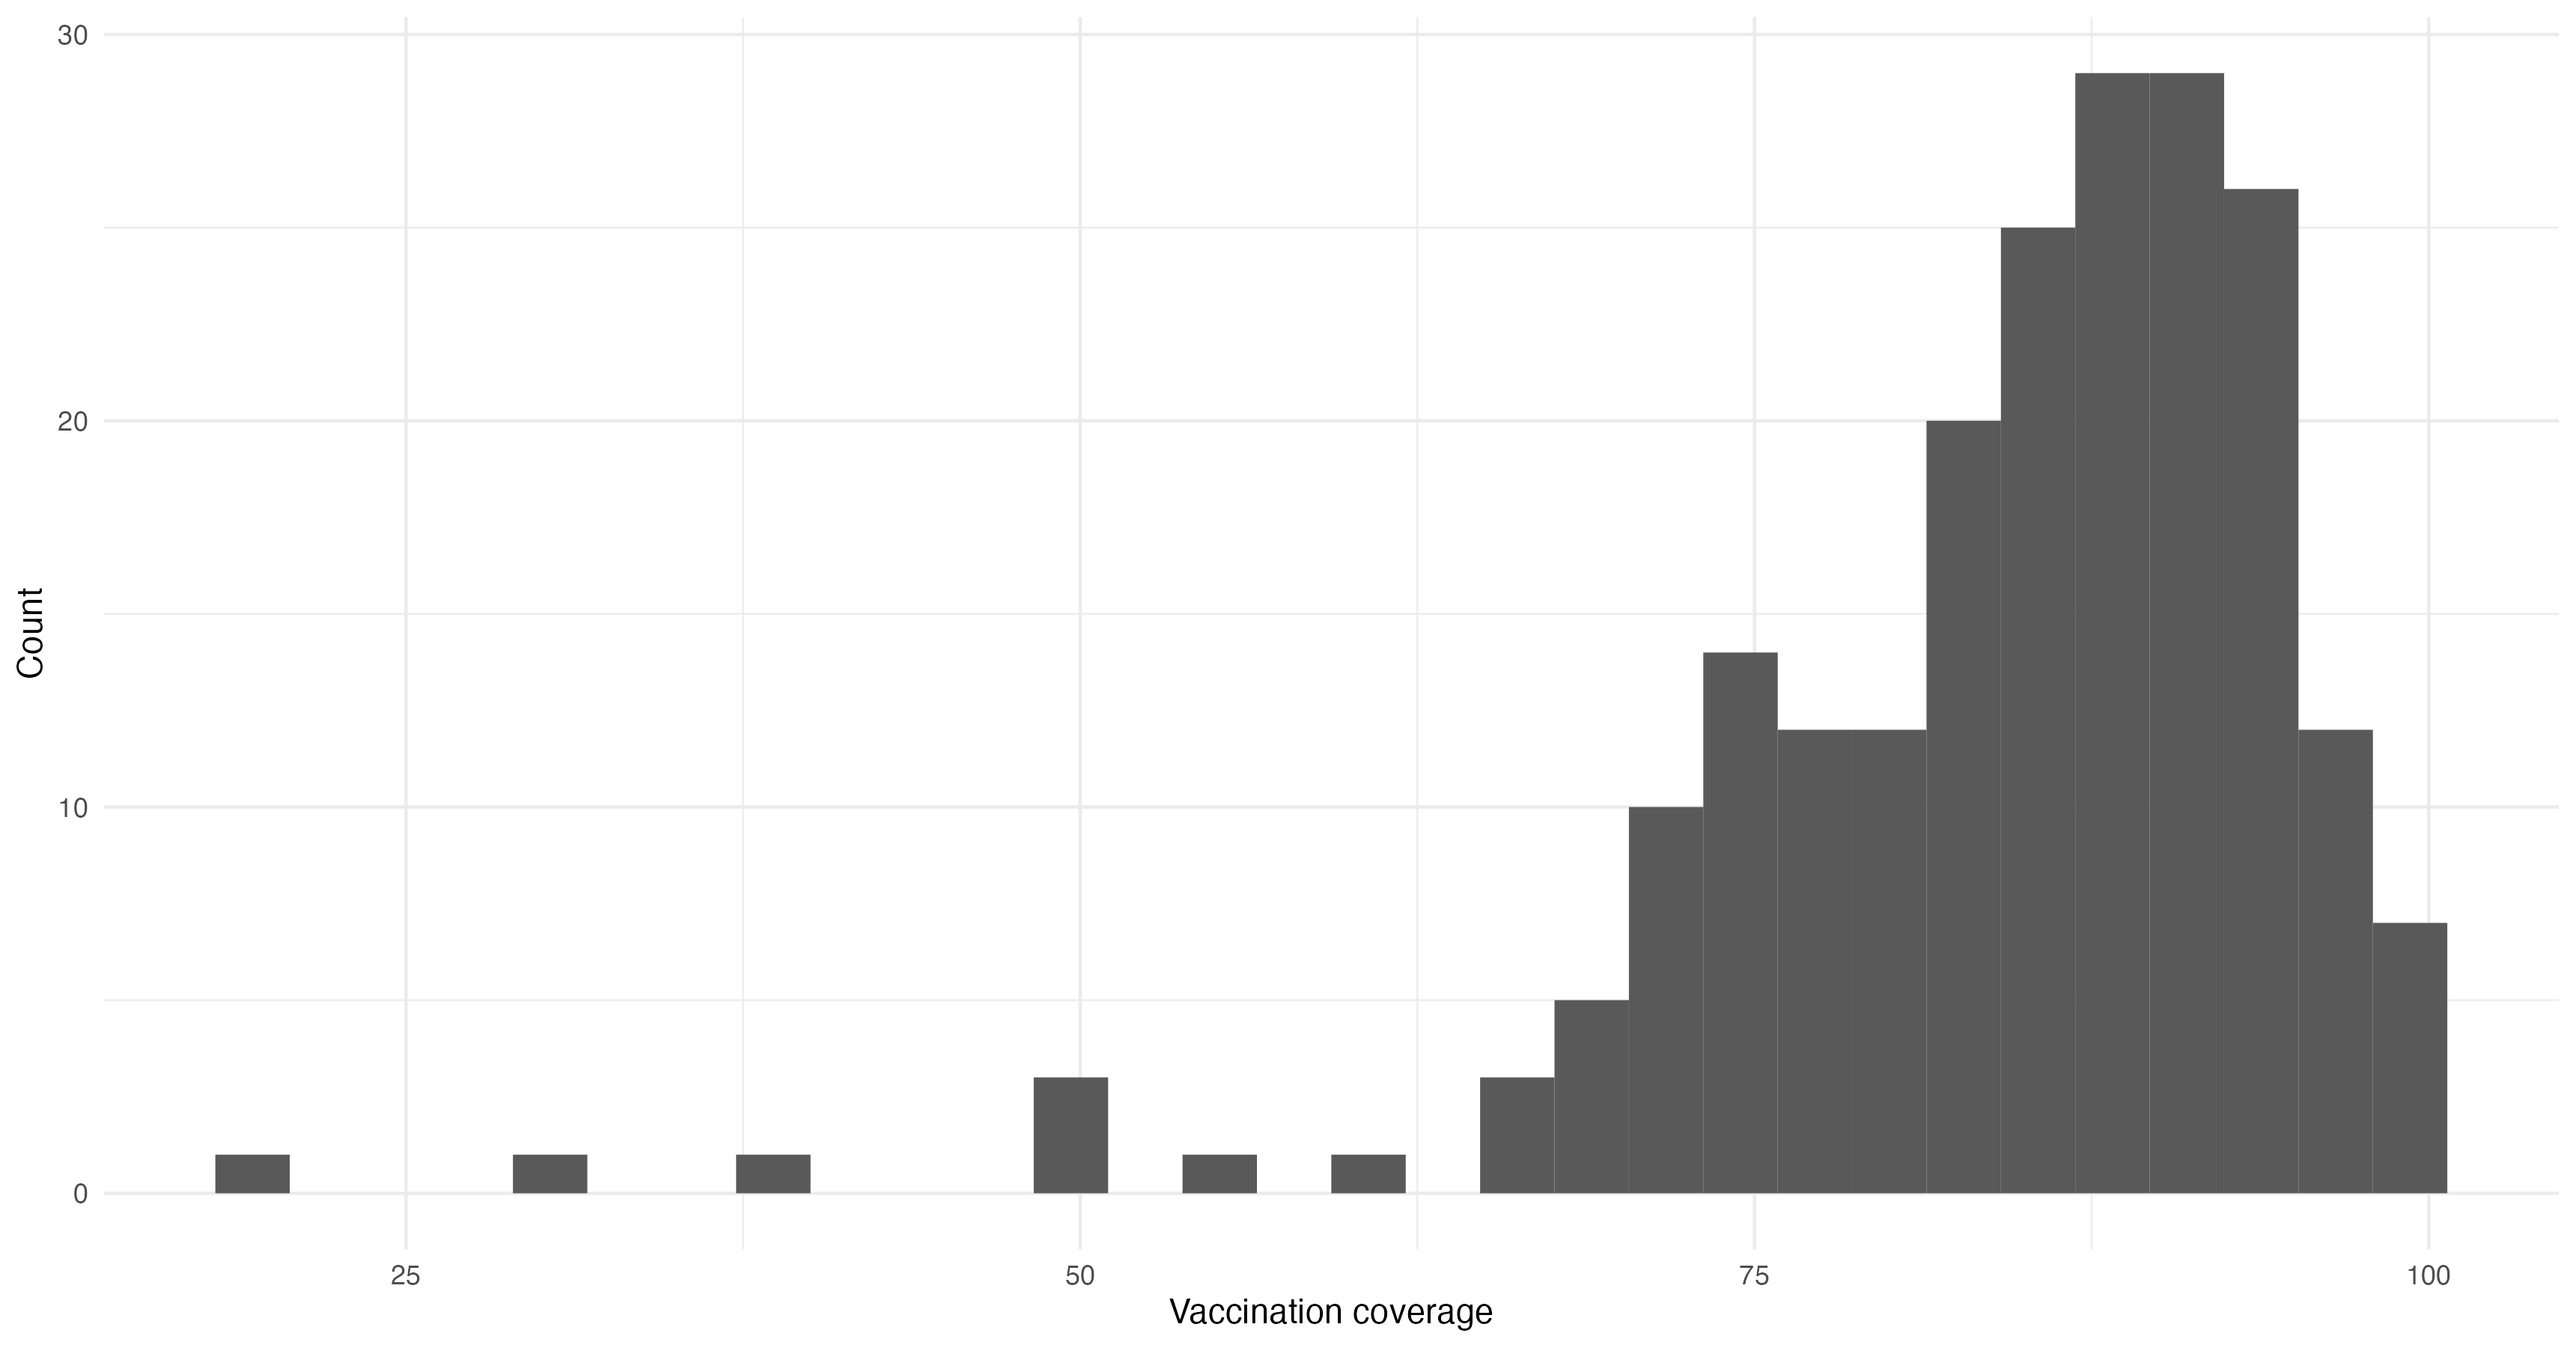
\includegraphics[width=\linewidth]{report-figs/f3.png}
\caption{VSB coverage}
\label{fig:vsbcov}
\end{figure}

Overall, Canadian vaccination for measles ranges from 60\% or below in some jurisdictions to above 90\% in others, with an overall high average of approximately 90\%. While measles has been considered eradicated in Canada since 1998, and high continuing levels of protection mean that endemic transmission has not been established, communities with low vaccination rates are at risk of outbreaks if introductions do occur.

\clearpage
\subsection{Modelling Approach}
We use a stochastic susceptible-exposed-infectious-recovered model with additional isolation compartments reflecting isolation of those who are susceptible and potentially exposed, or who have been infected but have not yet become symptomatic. The compartments are S: susceptible; E: exposed and not yet symptomatic (but some are already infectious prior to the onset of rash); I: symptomatic with rash (and infectious); R: recovered (immune); $Q_s$: not infected but isolating; $Q_r$: exposed and isolating or having received post-exposure prophylaxis (PEP). Susceptible individuals become infected at $a$ rate $b$ $(cE + I) S$, where $c$ reflects the fact that individuals become infectious approximately four days before the onset of rash. They are isolated at rate $q_s$ , and can be vaccinated via an additional public health vaccination effort at rate $v$. Exposed individuals are isolated or given PEP at rate $q_{spep}  = q_s + q_{pep}$, or enter the infectious (and transmitting) compartment at rate $k$, reflecting the (inverse of the) duration between infection and rash onset. Infectious individuals recover at rate $\gamma$ and are identified and isolated at rate $q_i$. Recovered individuals remain recovered; while immunity to measles may wane eventually, the waning rate is slow enough that in the $<1$ year time frame of the outbreaks considered here, we do not consider it.  We simulate the model with a Gillespie algorithm approach, computing the total rate for all events, sampling an exponential random variable to simulate the time until the next event, and then allocating which event occurs with the appropriate probability [REF].
We use two model populations: 1000, reflecting a school or other small setting in the 100s with surrounding households and immediate contacts, and 8000, reflecting a close-knit community, potentially with a lower-than-average vaccination rate [CITE Minnesota, other outbreaks].
We use reported outbreaks in high-vaccination countries, together with the natural history of measles, to roughly estimate parameters. We validate the model with comparison to past outbreak sizes and durations, though these are variable. We note that at 90\% vaccination measles is not spreading endemically despite regular introductions and occasional outbreaks. However, at 80\% vaccination we would anticipate that substantial public health interventions (additional vaccination, case identification, contact tracing, PEP, isolation of those who are exposed, and isolation of symptomatic individuals) are required to control outbreaks. These interventions are widely used in comparable jurisdictions to Canada.[CITE SOME OUTBREAKS].


\begin{table}[h!]
\centering
\caption{Parameters}
\label{tab:pars}
\begin{tabular}{p{2cm}p{4cm}p{6cm}p{5cm}}
\bf{Parameter} &
\bf{Value} &
\bf{Description} &
\bf{Reference or rationale} \\ \hline
$R_0$ &
  15 &
  Basic reproduction number. &
  \begin{tabular}[c]{@{}l@{}}Reported range 12-18.\\ {[}REFS{]}\end{tabular} \\ \hline
$c$ &
  0.3 &
  ``Exposed” individuals are infectious before onset of rash &
  4 days infectiousness prior to rash onset \\ \hline
$v$ &
  0.005 per day (strong); 0 (weaker) &
  Supplementary vaccination of susceptibles. Not all jurisdictions strongly encourage additional vaccination in the general population as an outbreak response. & British Columbia vaccination in 2019 outbreak (rough estimate) {[}REF{]} \\ \hline
$q_s$ &
  0.03 per day &
  Isolation of susceptible individuals following contact tracing, exposure notifications &
  See caption \\ \hline
  $q_{spep}$ &
  0.05 per day (strong); 0.04 (weak) &
  Post-exposure prophylaxis (PEP) plus isolation rate if PEP declined &
  See caption \\ \hline
$k$ &
  1/10 per day &
  Progression to rash onset &
  Course of infection (WHO) Rash onset at 7-18 days \\ \hline
$q_i$ &
  0.15 per day (strong); 0.1 per day (weaker) &
  Identification and isolation of symptomatic individuals &
  See caption \\ \hline
$\gamma $&
  1/4 per day &
  Recovery from symptoms and infectiousness &
  Infectious until 4 days after rash onset (WHO) \\ \hline
\end{tabular}
\end{table}

Rates corresponding to PEP and isolation of susceptible, exposed or symptomatic individuals are challenging to estimate, in part because outbreak reports rarely contain the required information. Briefly: $q_s$: it may take 2 days to find and contact susceptible people with exposure risk and advise isolating if they are unvaccinated; if half of them do so with 50\% effectiveness, this gives $q_s\approx0.03$.  $q_{pep}$: As with $q_s$, with two days to contact individuals who have been exposed to offer PEP, with partial uptake; then $q_{spep} = q_s + q_{pep}$. In Minnesota in a measles outbreak in 2016 (https://www.ncbi.nlm.nih.gov/pmc/articles/PMC5687591/), about 1/4 as many people received PEP as were excluded from childcare settings, though the denominators are not given. However this suggests that the rates of PEP and isolation/exclusion do not differ by orders of magnitude and that the PEP rate is lower. $q_i$: optimistically, within 2 days of rash onset at least half of individuals isolate with 60\% effectiveness (being unable to avoid contact with their household, and given the highly transmissible and airborne nature of measles and the potential need to seek healthcare).

\subsection{Validation}
Natural history parameters are relatively well-established for measles, but our intervention parameters are difficult to estimate. To ensure that our model creates realistic outbreaks for the kinds of population we consider, we compared model simulations to key features of measles outbreaks: size, duration, and controllability. It is well known that above 95\% vaccination measles will not spread, and the consistent experience in Canada since eradication in 1998 [CITE some PHAC THINGY] (and in similarly highly-vaccinated populations) suggests that even with very minor public health actions, outbreaks are not substantial in size at 90\% vaccination rates and are not large even at 85\%. However, once vaccination levels drop below that , at 80\% and below, outbreaks are more sizable. When sizable outbreaks occur in smaller settings and close-knit communities, they tend to last 60-70 days [LIST OF REFS] and range in size widely up to approximately 100 cases; the population size is rarely known or reported. Larger outbreaks occur, likely in larger populations and certainly over longer periods [Cite Lyon, New York].
Figure 4 shows an illustrative example outbreak; compare this to Figure 1 of [MINNESOTA 2016 report].
Model outbreaks similarly typically last 60-80 days and have comparable sizes to observed outbreaks, in as much as this comparison can be made without the necessary denominators (population sizes).

--------------- FIG 4 HERE --------




\end{document}
